%\documentclass[varwidth]{standalone}
\documentclass[10pt]{amsart}
\usepackage{amscd,amsxtra,color,amsthm}

\usepackage[all]{xy}
\usepackage{etex}
\usepackage{pictex}
\usepackage{graphicx}
\usepackage{tikz}
\usepackage[utf8]{inputenc} 
\usepackage[T1]{fontenc}
\usepackage[all]{xy}
\usepackage{etex}
\usepackage{pictex}
\usepackage{graphicx}
\usepackage{mathtools}
\DeclarePairedDelimiter{\ceil}{\lceil}{\rceil}
\DeclarePairedDelimiter{\floor}{\lfloor}{\rfloor}
\usepackage{comment}
\usepackage{enumitem}

\textheight=9in \textwidth=6.2in \topmargin=0in
\oddsidemargin=.15in \evensidemargin=.15in

\begin{document}
\parskip10pt
\parindent12pt
\baselineskip16pt

%%%%%%%%%%%%%%%%%%%%%%%%%%%%%%%%%%%%%%%%%%%%%%%%%%%%%%%%%%%%%%%%%%%%%%%%%%%%%%%%%%%%%%%%%%%%%%%%
%%  Definitions
%%%%%%%%%%%%%%%%%%%%%%%%%%%%%%%%%%%%%%%%%%%%%%%%%%%%%%%%%%%%%%%%%%%%%%%%%%%%%%%%%%%%%%%%%%%%%%%%

\def\G{\widetilde{G}}
\def\B{\widetilde{B}}
\def\T{\widetilde{T}}
\def\C{\mathbb{C}}
\def\A{\mathbb{A}}
\def\Z{\mathbb{Z}}
\def\R{\mathbb{R}}
\def\Q{\mathbb{Q}}
\def\N{\mathbb{N}}
\def\C{\mathbb{C}}
\def\F{\mathbb{F}}
\def\I{\mathbb{I}}
\def\H{\mathcal{H}}
\def\e{\varepsilon}
\def\s{\underline s}
\def\z{\zeta }
\def\vp{\varpi }
\def\O{\mathcal O}
\def\v{\upsilon }
\def\U{\Upsilon }
\def\p{\wp }
\def\p{\mathfrak{p}}
\def\B{\mathfrak{B}}


\newtheorem{theorem}{Theorem}%[section]
\newtheorem{lemma}[theorem]{Lemma}

%%%%%%%%%%%%%%%%%%%%%%%%%%%%%%%%%%%%%%%%%%%%%%%%%%%%%%%%%%%%%%%%%%%%%%%%%%%%%%%%%%%%%%%%%%%%%%%%
%%  Title Page
%%%%%%%%%%%%%%%%%%%%%%%%%%%%%%%%%%%%%%%%%%%%%%%%%%%%%%%%%%%%%%%%%%%%%%%%%%%%%%%%%%%%%%%%%%%%%%%%

\title{Byzantine Generals Problem}

\author{Graham Swain}

\begin{abstract}
    In this paper we explore the Byzantine Generals problem; an abstraction used to discuss the
    reliability of computing systems.
\end{abstract}

\maketitle

%%%%%%%%%%%%%%%%%%%%%%%%%%%%%%%%%%%%%%%%%%%%%%%%%%%%%%%%%%%%%%%%%%%%%%%%%%%%%%%%%%%%%%%%%%%%%%%%
%%  Introduction 
%%%%%%%%%%%%%%%%%%%%%%%%%%%%%%%%%%%%%%%%%%%%%%%%%%%%%%%%%%%%%%%%%%%%%%%%%%%%%%%%%%%%%%%%%%%%%%%%

\section{Introduction}

The Byzantine Generals Problem is a classic example that is used to abstract discussions of
computing systems. For a computing system to be reliable it must be able to deal with one or more
of its components failing. In the Byzantine Generals Problem each component is represented as a
general, the components that failed are traitorous generals. We will mostly be exploring when all the
components, or generals, have a direct line of communication, but we will briefly discuss about when
that is not the case.

The basis of the problem is we imagine that there are multiple divisions of the Byzantine army sieging
a city, each division led by a generals. The generals are only able to communicate by messengers. The
general needs to decide and agree on a plan. Unfortunately, some of the generals could be traitors,
trying to prevent the loyal generals from reaching an agreement. So the generals need  to have an
algorithm to guarantee that:

\begin{enumerate}[label={\Alph*.}]
    \item All loyal generals decide upon the same plan of action.
    \item A small number of traitors cannot cause the loyal generals to adopt a bad plan.
\end{enumerate}

The goal is to ensure that the loyal generals are able to agree on a reasonable plan, regardless
of traitorous generals. It is hard to quantify exactly what a ``bad'' plan is, but we do not have to
for our algorithm. How the generals reach a decision is more important. Let there be $n$ generals
and $v_i$ is the information communicated by the $i^{th}$ general. Each general has to use some method
of taking all of the plans communicated to them, $v_1,...,v_n$, and make a decision based off of them.
Having all of the generals use the same method of decision making would achieve Condition A.

Condition B can be met by using a robust decision making method. To simplify the problem we say that
the message can only be one of two orders ``ATTACK'' or ``RETREAT'', making $v_i$ General's $i$
opinion on which is the best option. Each general can take a majority vote of $v_1,...,v_n$ and let
whichever option wins be the ``best'' decision. This method only lets a small number of traitors
affect the result if the loyal generals are split fairly evenly between the two options, in which
case neither option could be deemed ``bad''. 

\pagebreak

To help ensure that Condition A and Condition B are met, we need to meet two other conditions:

\begin{enumerate}[label={\arabic{enumi}.}]
    \item Every loyal general must obtain the same information $v_1,...,v_n$.
    \item {
        If the $i^{th}$ general is loyal, then the value that they sends must be used by every loyal 
        general as the value of $v_i$.
    }
\end{enumerate}

\noindent Condition 1 could also be written as:
\begin{enumerate}[label={1$^{\prime}$.}]
    \item For every $i$, any two loyal generals use the same value of $v_i$.
\end{enumerate}

These are important because a loyal general cannot take a value $v_i$ at face value, because a
traitorous general could send different values of $v_i$ to different generals. Even though the
generals cannot necessarily trust every message, we must find a way to guarantee that loyal generals
use the values sent to them by other loyal generals.

Since Condition 1$^\prime$ and Condition 2 are both contingent on a single $v_i$ sent by the $i^{th}$
general, we can focus on how a single general sends values to others. We phrase this problem by 
referring to a commander sending messages to their lieutenants.

\emph{Byzantine Generals Problem.} A Commanding general must send an order to their $n - 1$ 
lieutenants such that:

\begin{enumerate}[label={IC\arabic{enumi}.}]
    \item All loyal lieutenants obey the same order.
    \item If the commander is loyal, then every loyal lieutenant obeys the order they sends.
\end{enumerate}

Conditions IC1 and Condition IC2 are called the interactive consistency conditions. If the commander
is loyal, then IC1 follows IC2. However, the commander can be a traitor.

%%%%%%%%%%%%%%%%%%%%%%%%%%%%%%%%%%%%%%%%%%%%%%%%%%%%%%%%%%%%%%%%%%%%%%%%%%%%%%%%%%%%%%%%%%%%%%%%
%%  Three Generals (Impossibility Result)
%%%%%%%%%%%%%%%%%%%%%%%%%%%%%%%%%%%%%%%%%%%%%%%%%%%%%%%%%%%%%%%%%%%%%%%%%%%%%%%%%%%%%%%%%%%%%%%%
\section{Three Generals}

When sending only oral messages, at least two thirds of the lieutenants must be loyal for any
solution to work. The distinction of oral message is important, as it means that the contents of a
message is completely up to sender. So a traitorous sender can send any message they want.

We will look at the simplest form of this problem, where there are three generals (one commander and
two lieutenants). There are two possible orders: "ATTACK" or "RETREAT". No solution can exist for
this if there is even a single traitor.

\noindent \emph{Situation 1.} The commander is loyal, but one of the lieutenants is a traitor.

\begin{minipage}{.95\textwidth}%
    The commander sends out the command ATTACK to both lieutenants. Both lieutenants rely the order
    they receive to the other, but since one lieutenant is a traitor, they rely the message RETREAT.
    The loyal lieutenant receives the set of orders: {ATTACK, RETREAT}, there is no way for him
    to decide which is the correct order. 
\end{minipage}%

\pagebreak

\begin{figure}[h!]
    \centering
    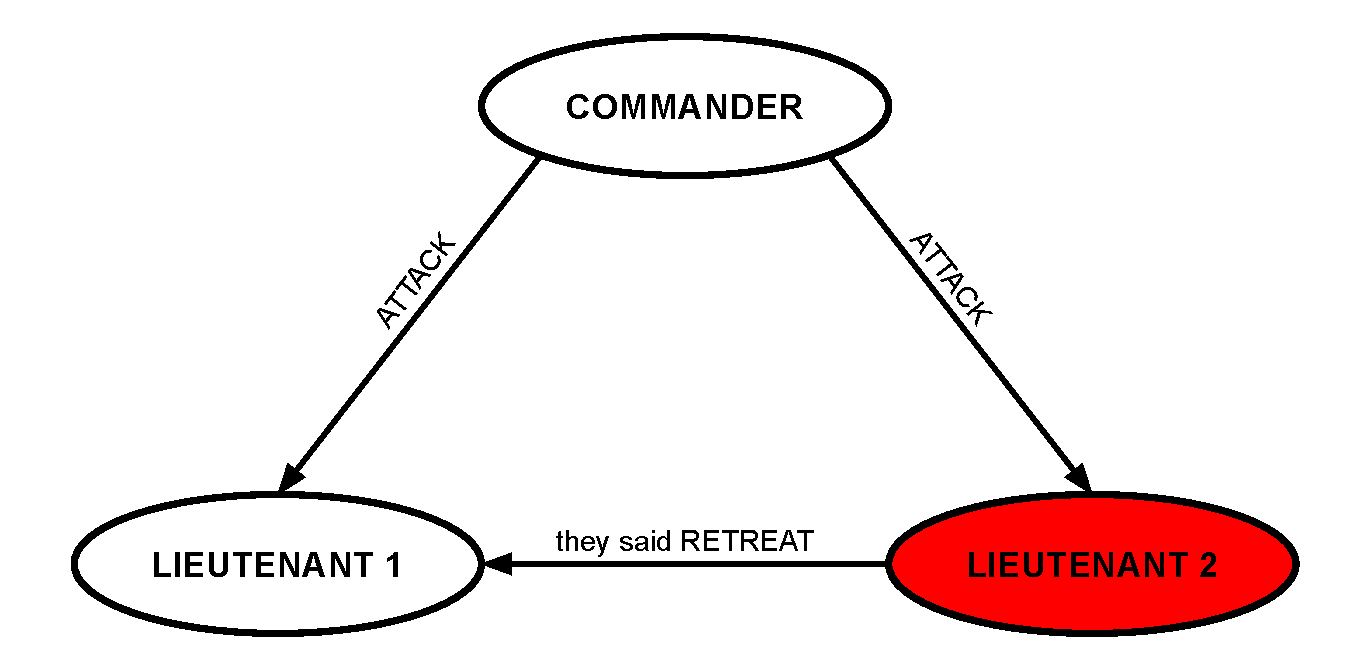
\includegraphics[scale=.6]{../figures/three_generals_loyal_commander.pdf}
    \caption{Three General Problem with a loyal Commander.}
\end{figure}


\noindent \emph{Situation 2.} The commander is not loyal, both lieutenants are.

\begin{minipage}{.95\textwidth}%
    The commander sends ATTACK to Lieutenant 1 and RETREAT to Lieutenant 2. Since they are both loyal
    they rely the commands to each other. Lieutenant 1 receives the set of orders: {ATTACK, RETREAT}.

    Since Lieutenant 1 receives the set of orders: {ATTACK, RETREAT} in both situations, there is no
    way for them to know who they traitor is, so they follows their commander's orders to attack in 
    both situations, regardless of if the commander is a traitor.

    We can make a similar argument that Lieutenant 2 must follow the RETREAT command in the second
    situation. This violates IC1 since the two loyal lieutenants obey different orders. 
\end{minipage}%

\begin{figure}[h!]
    \centering
    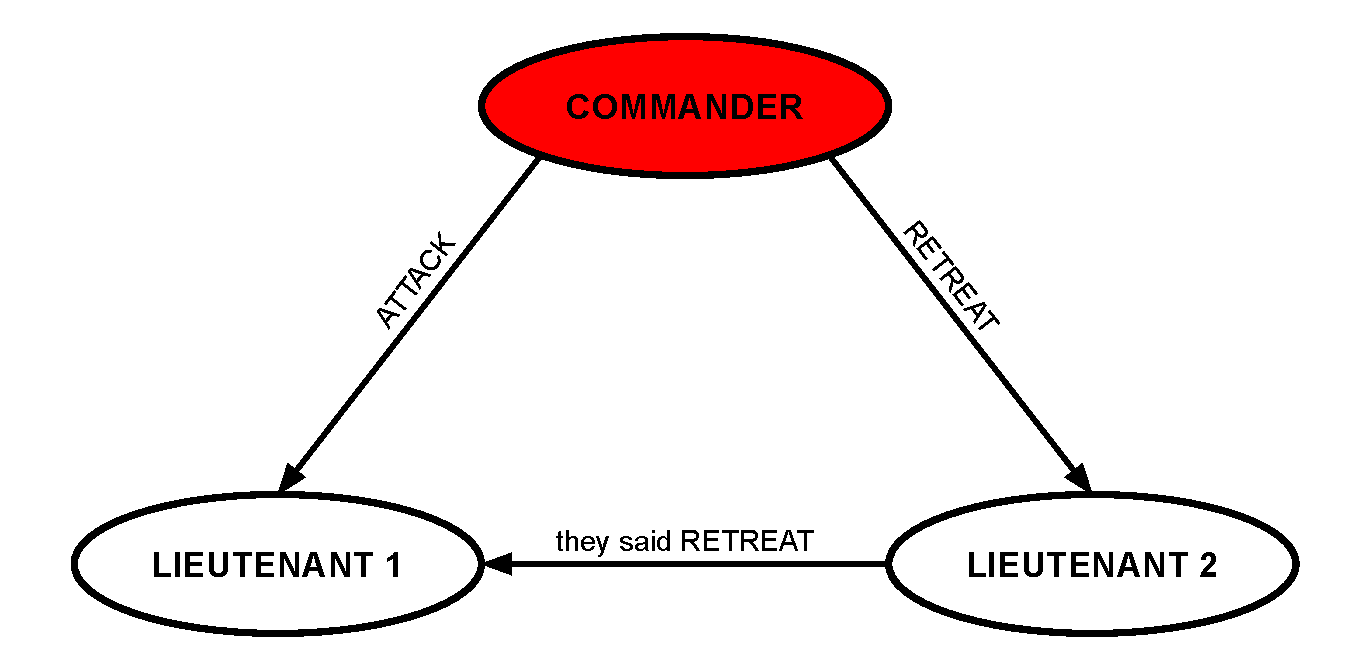
\includegraphics[scale=.6]{../figures/three_generals_unloyal_commander.pdf}
    \caption{Three General Problem with a disloyal Commander.}
    \label{fig:3gen_comm}
\end{figure}

The authors have a formal solution for the three generals problem in their 1980 paper "Reaching 
Agreement in the Presence of Faults" if you want to read more about it. For the purposes of this
paper it is only important to know that no solution exists for three generals if there is a single
traitor.

Using the result that a single traitor can disrupt the the three generals problem, we can show that
no solution exists with less than $3m+1$ generals and $m$ traitors. To help differentiate between
the problems, the generals from the three generals problem will be referred to as Byzantine generals
and the generals from the assumed solution will be referred to as Albanian generals.

\begin{proof}
    We want to prove that no solution exists with $n < 3m + 1$ generals with $m$ traitors and $n > 3$.
    We will prove this by contradiction. 

    Assume that a solution exists for $3m$ or less Albanian generals. We will show a solution exits
    for three Byzantine generals with a single traitor. Each Byzantine general represents at most 
    $m$ Albanian generals. Since the Albanian commander needs to be represented as well, the
    Byzantine commander represents the Albanian commander as well as at most $m-1$ Albanian lieutenants.
    We know that there is a single Byzantine traitor. Since each Byzantine general represents at
    most $m$ Albanian generals, we know there is at most $m$ Albanian traitors. The assumed solution
    means that IC1 and IC2 is true for the Albanian generals. Since each Albanian general is 
    represented by a Byzantine general, then IC1 and IC2 must also be true for the Byzantine generals,
    which we know is impossible, forming a contradiction.
\end{proof}

%%%%%%%%%%%%%%%%%%%%%%%%%%%%%%%%%%%%%%%%%%%%%%%%%%%%%%%%%%%%%%%%%%%%%%%%%%%%%%%%%%%%%%%%%%%%%%%%
%%  Oral Solution 
%%%%%%%%%%%%%%%%%%%%%%%%%%%%%%%%%%%%%%%%%%%%%%%%%%%%%%%%%%%%%%%%%%%%%%%%%%%%%%%%%%%%%%%%%%%%%%%%
\section{Oral Solution}

The above section shows that we need at least $3m+1$ generals to solve the Byzantine Generals Problem
using oral messages, with m traitors.  In this section we will create an algorithm that will work for
$3m+1$ or more generals. We make three assumptions to define an oral message:
\begin{enumerate}[label={A\arabic{enumi}.}]
    \item Every message that is sent is delivered correctly.
    \item The receiver of a message knows who sent it.
    \item The absence of a message can be detected.
\end{enumerate}

These assumptions each help prevent foul play by traitorous generals. A1 prevents traitor from
stopping messages from being received. A2 make it to where a traitor cannot impersonate another.
A3 stops traitors who try and prevent a decision from being made by not sending messages.

For this problem we assume that every general is able to send a message to every other general. That
is often not the cased and will be discussed in a later section. We also assume that every loyal 
general completes their algorithm. In the case of a traitorous general who does not send any orders
at all, we assume that lieutenants default to the RETREAT order.

We will define an algorithm for oral messages OM($m$), for all nonnegative integers $m$. In this algorithm
a commander sends an order to $n-1$ lieutenants. OM($m$) will solve the Byzantine Generals Problem for
$3m+1$ more generals when there is at most $m$ traitors.

As stated above, when a general receives a message, or a value, from a general, we denote it as $v_i$
for the $i^{th}$ general. Whenever a general has a set of all the messages, $v_i,...,v_n$, they use a 
majority function majority($v_i,...,v_n$) = $v$, $v$ being the decision the lieutenant comes too. Two choices 
for deciding the majority listed in the paper are:
\begin{enumerate}[label={\arabic{enumi}.}]
    \item {
        The majority value among the $v_i$ (the value that occurs the most) if one exists, or default 
        to the value RETREAT.
    }
    \item The median value of the $v_i$, if the set is ordered.
\end{enumerate}

The algorithm is recursive, so starts with a base case of OM(0) and uses the majority function.

\noindent\emph{Algorithm OM(0)}
\vspace{-10pt}
\begin{enumerate}[label=\arabic{enumi}.]
    \item The commander sends their value to every lieutenant.
    \item {
        Each lieutenant uses the value they received from the commander. If they received no value, 
        default to RETREAT.
    }
\end{enumerate}

\noindent\emph{Algorithm OM($m$), $m$ > 0}
\vspace{-10pt}
\begin{enumerate}[label=\arabic{enumi}.]
    \item The commander sends their value to every lieutenant.
    \item For each $i$,
    \begin{enumerate}[label={\alph*.}]
        \item {
            Lieutenant $i$ receives a value $v_i$ from the commander. Default to RETREAT if they receive
            no value.
        }
        \item {
            Lieutenant $i$ acts as the commander in OM($m-1$) to send the message to each of the remaining
            $n-2$ lieutenants.
        }
    \end{enumerate}
    \item For each $i$, and each $j$ not equal to $i$,
    \begin{enumerate}[label={\alph*.}]
        \item {
            let $v_j$ be the value Lieutenant $i$ received from Lieutenant $j$ in step (2b). Default to 
            RETREAT if Lieutenant $i$ received no value from Lieutenant $j$.
        }
        \item Lieutenant $i$ uses the value $majority(v_1,...,v_{n-1})$.
    \end{enumerate}  
\end{enumerate}

Let's look at an example with four generals and one traitor, or $n=4$ and $m=1$. There are two
situations, where one of the lieutenants is a traitor or where the commander is a traitor.

\noindent \emph{Situation 1.} Lieutenant 3 is a traitor.

\begin{minipage}{.95\textwidth}%
    In the first step of the algorithm OM(1), the commander sends the order $x$ to all three lieutenants.
    In the second step, Lieutenant 1 sends the value $x$ to Lieutenant 2 using OM(0). Lieutenant 3 sends
    $y$ to Lieutenant 2. In step 3, Lieutenant 2 has the set of orders $v_1=v_2=x$ and $v_3=y$. Using
    $majority(x, x, y) = x$, Lieutenant 2 follows the order $x$ sent to him by the commander. We can use
    a similar process to find that Lieutenant 1 also follows order $x$. So both loyal lieutenants followed
    the order of their loyal commander. This satisfies IC1 and IC2.
\end{minipage}%

\begin{figure}[h!]
    \centering
    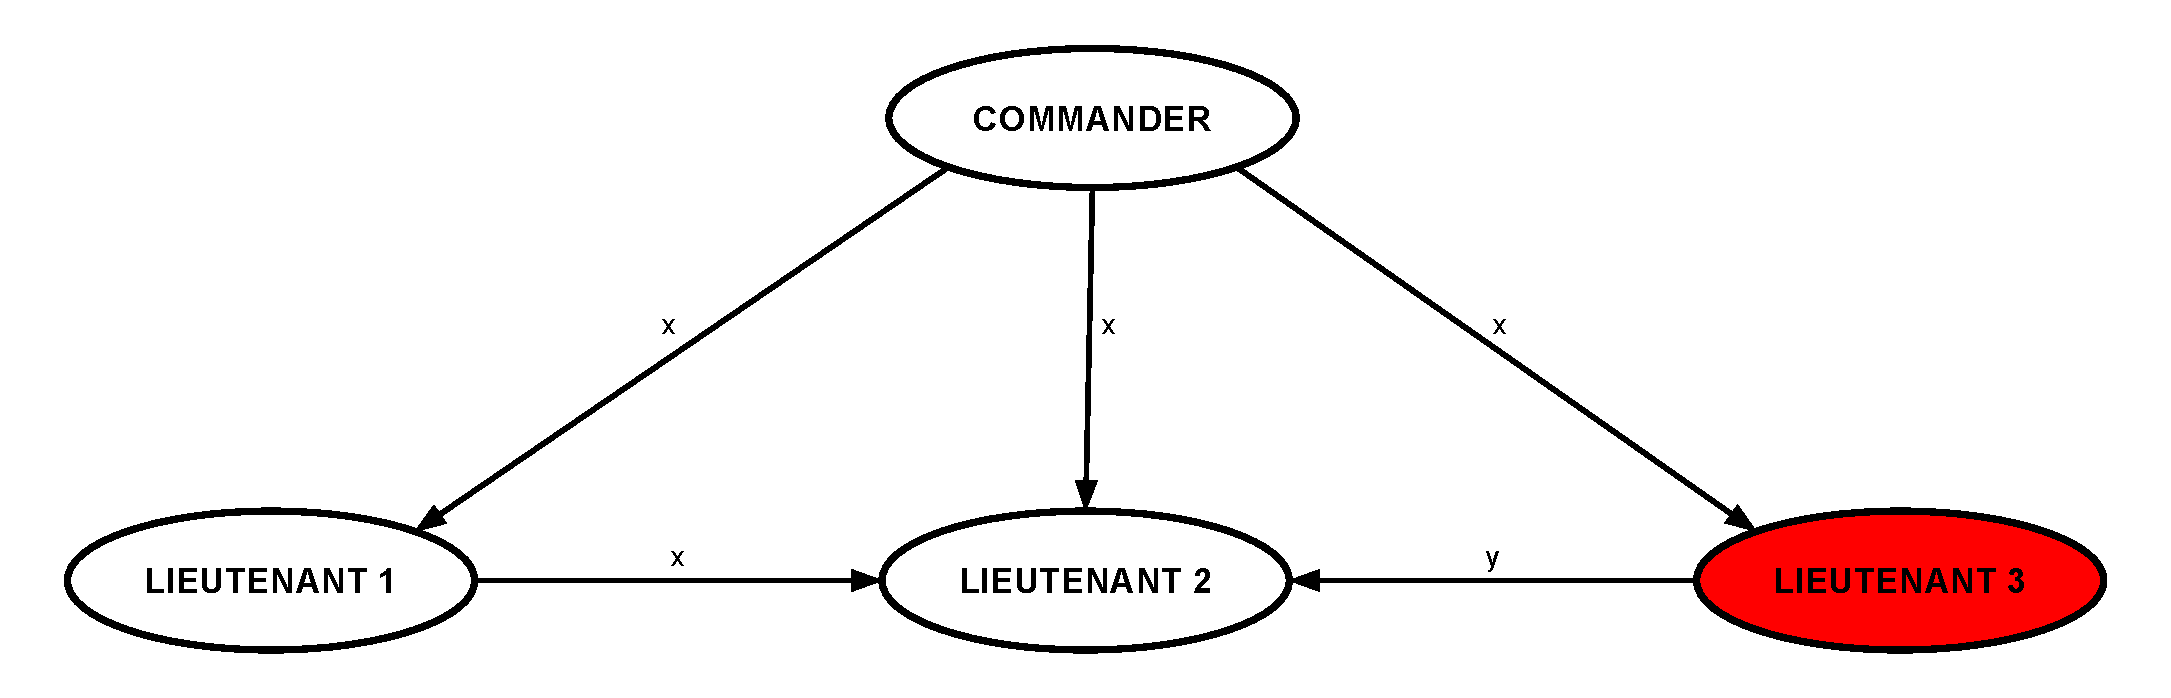
\includegraphics[scale=.4]{../figures/oral_messages_OM(1)_loyal_commander.pdf}
    \caption{OM(1) with a disloyal lieutenant.}
\end{figure}

\pagebreak

\noindent \emph{Situation 2.} The commander is a traitor. 

\begin{minipage}{.95\textwidth}%
    The commander sends the arbitrary orders $x$, $y$, $z$ to Lieutenants 1, 2, 3 respectively. In step 2 each
    lieutenant sends the order they got to the others. In step 3 each lieutenant ends up with $v_1=x$,
    $v_2=y$, $v_3=z$ and the majority function $majority(x,y,z)$. So they each will follow the same order
    regardless of if the values of $x$, $y$, $z$ are equal to one another or not. This satisfies IC1.
\end{minipage}%

\begin{figure}[h!]
    \centering
    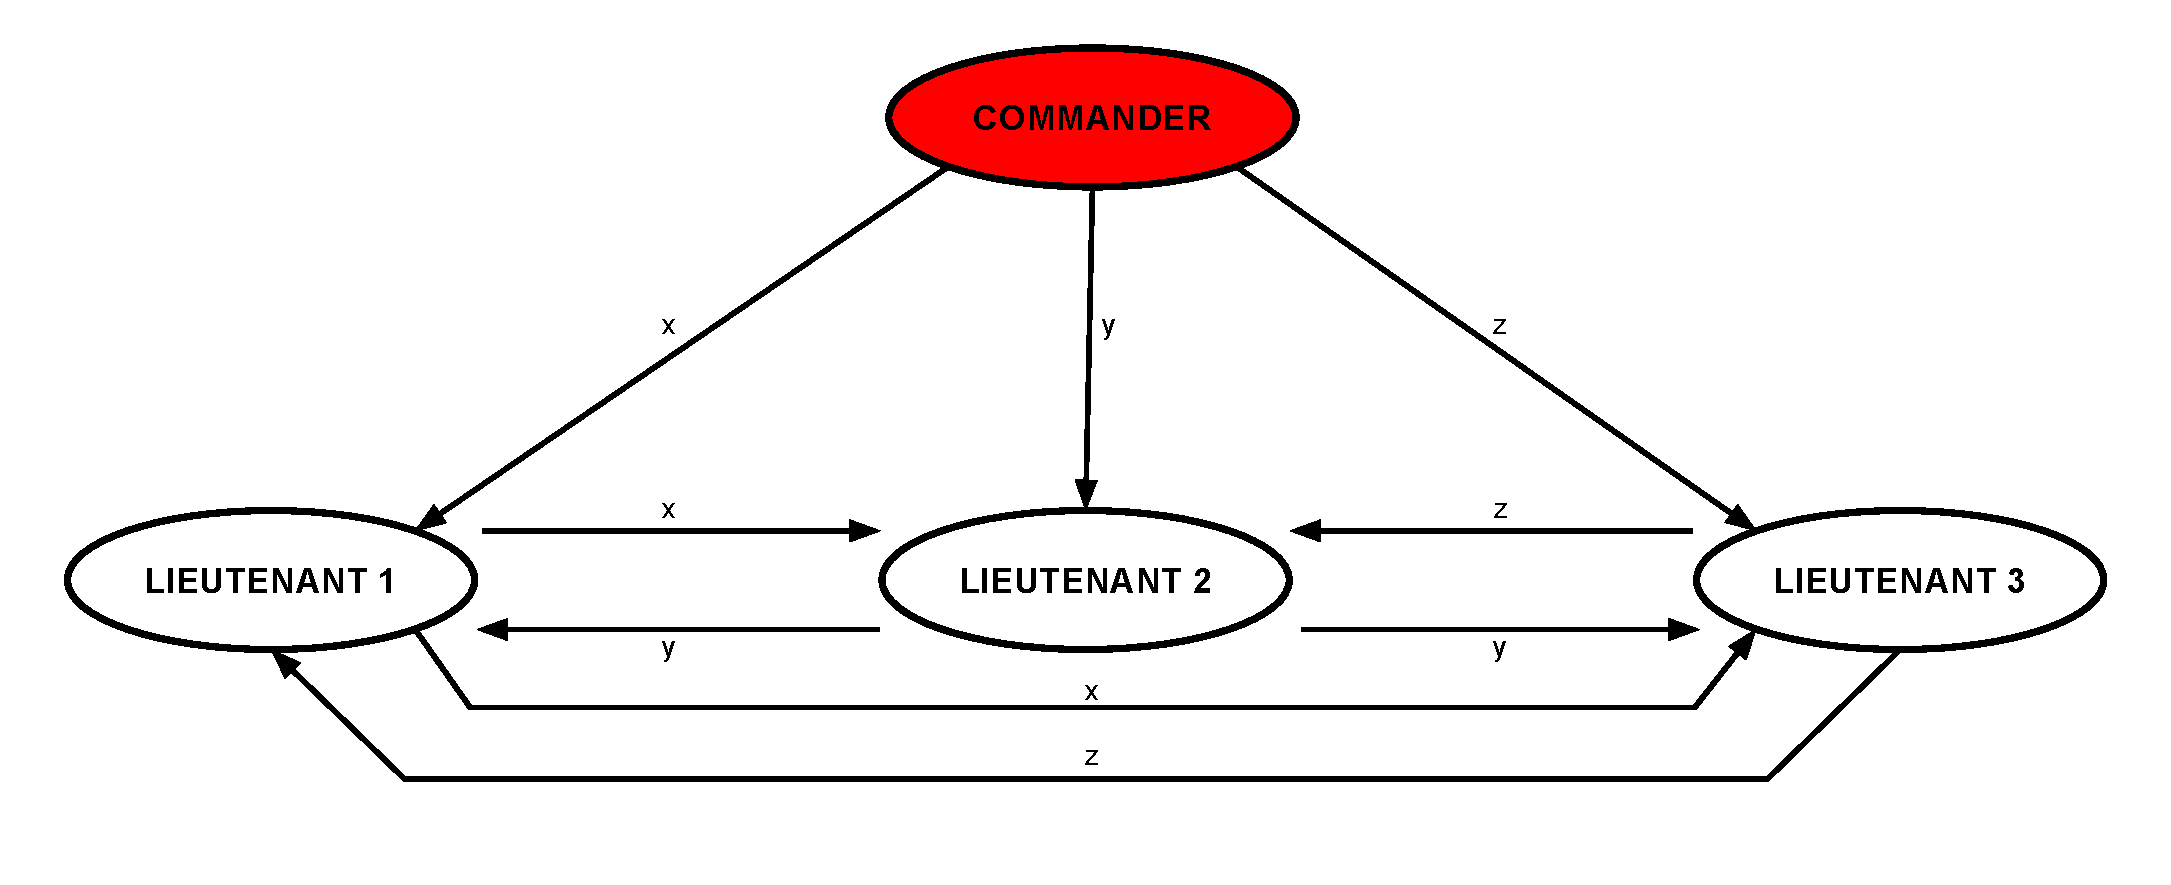
\includegraphics[scale=.4]{../figures/oral_messages_OM(1)_unloyal_commander.pdf}
    \caption{OM(1) with a disloyal lieutenant.}
\end{figure}

Before we can prove that the algorithm OM($m$) works for an arbitrary $m$, we first need to prove the
following lemma.

\begin{lemma}
    \label{lemma1}
    For any $m$ and $k$, Algorithm OM($m$) satisfies IC2 if there are more than $2k+m$ generals and at
    most $k$ traitors.
\end{lemma}

\begin{proof}
    We will prove this by induction on m. \\
    IC2 only cares when the commander is loyal. Using A1, we know that every message is delivered
    correctly. OM(0) works if the commander is loyal, since the lieutenants all receive the order. So
    it holds true for $m$ = 0. \\
    Now we assume it is true for $m-1$, $m>0$, and will prove for $m$. \\
    In step 1, the loyal commander sends a value v to all $n-1$ lieutenants. Each loyal lieutenant calls
    OM($m-1$) with $n-1$ generals. We know $n>2k+1$, so we know $n-1>2k+m-1$ or $n-1>2k+(m-1)$. We use the inductive
    hypothesis and conclude that every loyal lieutenant gets $v_j=v$ for each loyal Lieutenant $j$. Since
    $n-1>2k+(m-1)\geq2k$ and we know there is at most $k$ traitors, the majority of $n-1$ lieutenants are loyal.
    So every loyal lieutenant gets $v_i=v$ for a majority of the $n-1$ values $i$. This gives him 
    $majority(v_1,...,v_{n-1})$ in step 2. This proves IC2.
\end{proof}

\begin{theorem}
    \label{theorem1}
    For any $m$, Algorithm OM($m$) satisfies conditions IC1 and IC2 if there are more than $3m$ generals 
    and at most $m$ traitors.
\end{theorem}

\begin{proof}
    We prove this using induction on m. \\
    It is simple to see that OM(0) satisfies IC1 and IC2 if there are no traitors.
    Assume the theorem is true for OM($m-1$) and prove it for OM($m$), when $m>0$.

    \begin{minipage}{.8\textwidth}%
        \textbf{Case 1.} The commander is loyal. \\
        Use Lemma 1 and set $k$ equal to $m$.
        \[ n > 2k + m \] 
        \[ n > 3k. \]
        We see that OM($m$) satisfies IC2, and IC1 follows if the commander is loyal.
    \end{minipage}%

    \begin{minipage}{.8\textwidth}%
        \textbf{Case 2.} The commander is a traitor. \\
        We know there is at most $m$ traitors, since one is the commander, there is at most $m-1$
        traitorous lieutenants. We also know that there are more than $3m$ generals, therefore there
        are more than $3m-1$ lieutenants. $3m-1 > 3(m-1)$. We can apply the inductive hypothesis and
        see that O($m-1$) meets both IC1 and IC2. Since IC2 is satisfied, we know every loyal
        lieutenant receives the same set of values $v_1,...v_{n-1}$. Therefore they come to the same
        value using the $majority(v_1,...,v_{n-1})$ function, proving IC1.
    \end{minipage}%

    This proves that OM($m$) satisfies IC1 and IC2 if there is more than $3m$ generals.
\end{proof}

%%%%%%%%%%%%%%%%%%%%%%%%%%%%%%%%%%%%%%%%%%%%%%%%%%%%%%%%%%%%%%%%%%%%%%%%%%%%%%%%%%%%%%%%%%%%%%%%
%%  Signed Messages 
%%%%%%%%%%%%%%%%%%%%%%%%%%%%%%%%%%%%%%%%%%%%%%%%%%%%%%%%%%%%%%%%%%%%%%%%%%%%%%%%%%%%%%%%%%%%%%%%
\section{Signed Messages}

So far we have been looking at oral, unsigned messages. This make finding a solution to the Byzantine
Generals Problem more difficult because it allows the traitorous generals to lie. Restricting a
traitor's ability to lie would make solving the problem easier. In this section we will explore that
by having each general send signed messages with a signature that cannot be forged. To do this we
need more assumptions:

\begin{enumerate}[label={A4.}]
    \item {
        \begin{enumerate}[label={(\alph*)}]
            \item {
                A loyal general's signature cannot be forged, and any alterations of the contents of
                their signed messages can be detected.
            }
            \item Anyone can verify the authenticity of a general's signature.
        \end{enumerate}
    }
\end{enumerate}

No assumptions are made about traitors' signature. It is possible for traitors to forge another
traitor's signature and to collude in that manner.

This new algorithm is able to cope with $m$ traitors for any amount of generals, due to the messages
now being signed. The authors do note that it does not make much sense for less than $m+2$ generals.

In this new algorithm, every when the commander sends an order they sign it. So each lieutenant receives
an order with the commanders signature. They then add their signature to the message before sending
it to the other lieutenants. Since each lieutenant will receive multiple messages with orders, we
need a choice function to decide which order to follow. The only requirements for such a function are:

\begin{enumerate}[label={\arabic{enumi}.}]
    \item If the set $V$ consists of the single element $v$, then $choice(V) = v$.
    \item $choice(\emptyset)=$ RETREAT, where $\emptyset$ is the empty set.
\end{enumerate}

\noindent The actual decision for deciding between different orders, as it will differ between
implementations. It only matters that all loyal generals use the same decision making process.

In the algorithm we denote the value $x$ signed by General $i$ as $x:i$. That means $v:j:i$ would be the 
value $v$ signed by General $j$ and then signed by General $i$. Each General $i$ maintains a set of properly
signed orders $V_i$. A loyal commander should never have more than one element in $V_i$. $V_i$ is specifically
the set of orders a general has received, not the set of messages they have received.

\noindent\emph{Algorithm SM($m$), $m$ > 0} \\
Initially $V_i=\{\}$
\vspace{-10pt}
\begin{enumerate}[label=\arabic{enumi}.]
    \item The commander signs and sends their value to every lieutenant.
    \item For each $i$,
    \begin{enumerate}[label={\alph*.}]
        \item {
            If Lieutenant $i$ receives a message from the commander of form $v:0$ and they have not received
            any other order, then:
            \begin{enumerate}[label=\roman*.]
                \item they set $V_i=\{v\}$.
                \item they send the message $v:0:i$ to every other lieutenant.
            \end{enumerate}
        }
        \item {
            If Lieutenant $i$ receives a message of the form $v:0:j_1:...:j_k$ and $v$ is not in $V_i$, 
            then:
            \begin{enumerate}[label=\roman*.]
                \item they add $v$ to $V_i$.
                \item {
                    if $k < m$, then they send the message $v:0:j_1:...:j_k:i$ to every other lieutenant,
                    except for $j_1,...,j_k$.
                }
            \end{enumerate}
        }
        \item {
            For each $i$, when Lieutenant $i$ receives no more messages, they follow the result from 
            $choice(V_i)$.
        }
    \end{enumerate}
    
\end{enumerate}

\begin{figure}[h!]
    \centering
    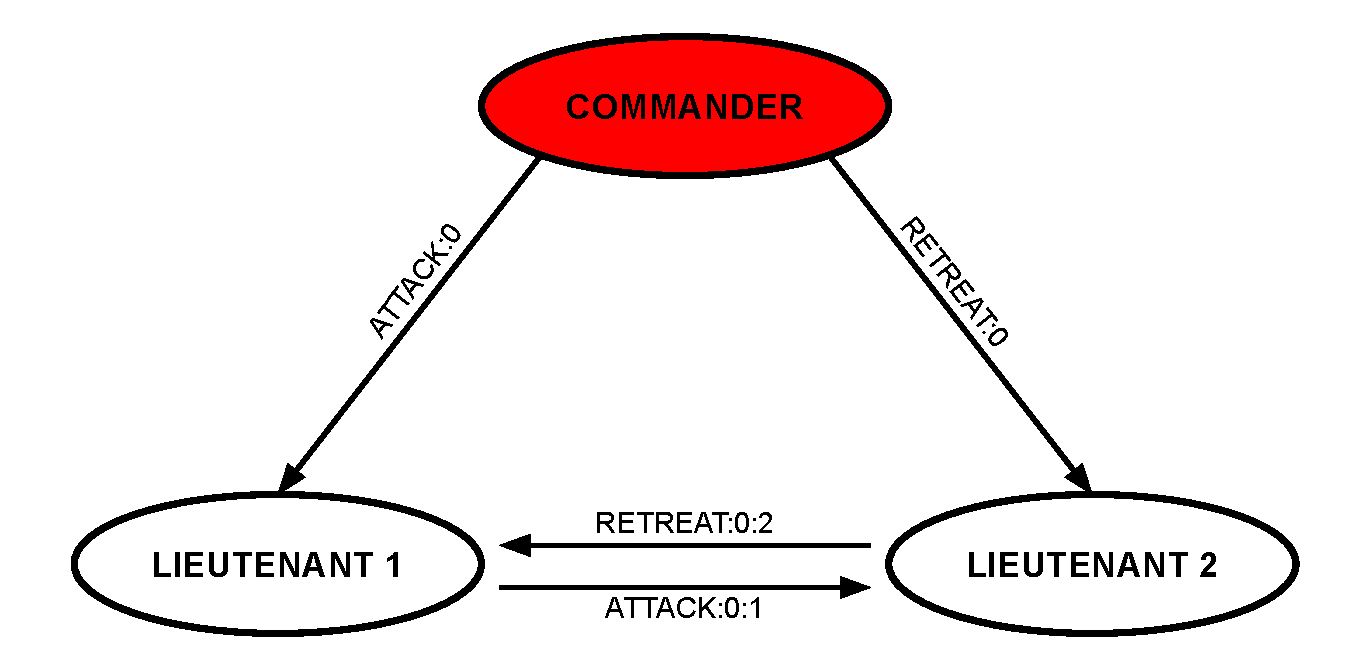
\includegraphics[scale=.55]{../figures/signed_messages_disloyal_commander.pdf}
    \caption{SM(1) with a disloyal lieutenant.}
    \label{fig:signed}
\end{figure}

We can look at Figure \ref{fig:signed} to see how signed messages can make the problem
easier. The traitorous commander sends conflicting commands to their two lieutenants. Since the lieutenants
are loyal, they rely the message they receive, adding their own signatures. In step (3) the lieutenants
have the sets of orders $V_1=V_2={ATTACK, RETREAT}$. The difference between this and Figure \ref{fig:3gen_comm}
is the lieutenants know that the commander sent different commands, so they are the traitor.

\pagebreak

Now to prove that SM($m$) offers a valid solution.

\begin{theorem}
    \label{theorem2}
    For any $m$, Algorithm SM($m$) solves the Byzantine Generals Problem if there are at most $m$
    traitors.
\end{theorem}

\begin{proof}
    We first prove IC2. If the commander is loyal, they sends their signed order $v:0$ to every lieutenant
    in step (1). This means that every loyal lieutenant will receive the order $v$ in step (2a). According
    to assumption A4, a loyal general's signature cannot be forged. So no traitorous general can
    forge a message $v':0$, so a loyal lieutenant cannot receive any additional orders in step (2b). 
    Every loyal Lieutenant $i$ will contain the single order $v$ in the set $_Vi$. In step three they will
    follow $v$ in accordance with the first property of the choice function. This proves IC2.

    Now we prove IC1. We only need to prove IC1 when the commander is a traitor because IC1 follows
    IC2 when the commander is loyal. Two loyal generals, $a$ and $b$, will follow the same order in step (3) if the
    set of orders they receive in step (2), $V_a$ and $V_b$, are the same. We need to prove that if $a$ puts an order $v$
    in $V_a$ then $b$ must put the same order $v$ in $V_b$. There are two possibilities in step (2). The first
    option is a receives the message $v:0$ directly from the commander. They adds the order to $V_a$, step (2ai),
    then sends the message $v:0:a$ to every other general, including $b$. So we know $b$ receives the order $v$.
    The other option is if $a$ receives a message in the form of $v:0:j_1:...:j_k$. If $b$ is contained in
    $j_1...j_k$, then we know $b$ has already received the order (due to A4). If not, we must consider two
    cases:
    \begin{enumerate}[label=\arabic{enumi}.]
        \item $k<m$. In this case, a will send the message $v:0:j_1:...:j_k:a$ to $b$, so we know $b$ receives $v$.
        \item {
            $k = m$. We know the commander is a traitor, which means there is at most $m - 1$ traitorous
            lieutenants. This means at least one of the lieutenants $j_1,...,j_m$ is loyal. Since
            loyal lieutenants follow the algorithm, we know that the loyal lieutenant must have sent
            the value $v$ to $j$ when they had first received it.
        }
    \end{enumerate}
    This proves that SM($m$) solves the Byzantine Generals Problem.
\end{proof}

%%%%%%%%%%%%%%%%%%%%%%%%%%%%%%%%%%%%%%%%%%%%%%%%%%%%%%%%%%%%%%%%%%%%%%%%%%%%%%%%%%%%%%%%%%%%%%%%
%%  Missing Communication Paths
%%%%%%%%%%%%%%%%%%%%%%%%%%%%%%%%%%%%%%%%%%%%%%%%%%%%%%%%%%%%%%%%%%%%%%%%%%%%%%%%%%%%%%%%%%%%%%%%
\section{Missing Communication Paths}

So far we have assumed that every general could message every other general directly. In the real 
world that is very rarely the case. Now we will explore extensions of OM($m$) and SM($m$) that can handle missing communication
links. To do this we will represent the generals as nodes in a simple, undirected graph, $G$, with the edges
representing lines of communication. 

To explore this new twist on the problem, we first need some definitions.

\noindent {\bf Definition.} { 
    A set of nodes $\{i_1,...,i_p\}$ is said to be a \textbf{regular set of neighbors} of a node $i$ if 
    \vspace{-10pt}
    \begin{enumerate}[label=\roman*.]
        \item each $i_j$ is a neighbor of $i$, and
        \item {
            for any general $k$ different from $i$, there exists paths $\gamma_{j,k}$ from $i_j$ to $k$ not passing
            through $i$ such that any two different paths $\gamma_{j,k}$ have no node in common other than $k$.
        }
    \end{enumerate}
}

\noindent {\bf Definition.} { 
    The graph $G$ is said to be \textbf{p-regular} if every node has a regular set of neighbors 
    consisting of $p$ distinct nodes.
}

\begin{figure}[h!]
    \begin{minipage}{.5\textwidth}
        \centering
        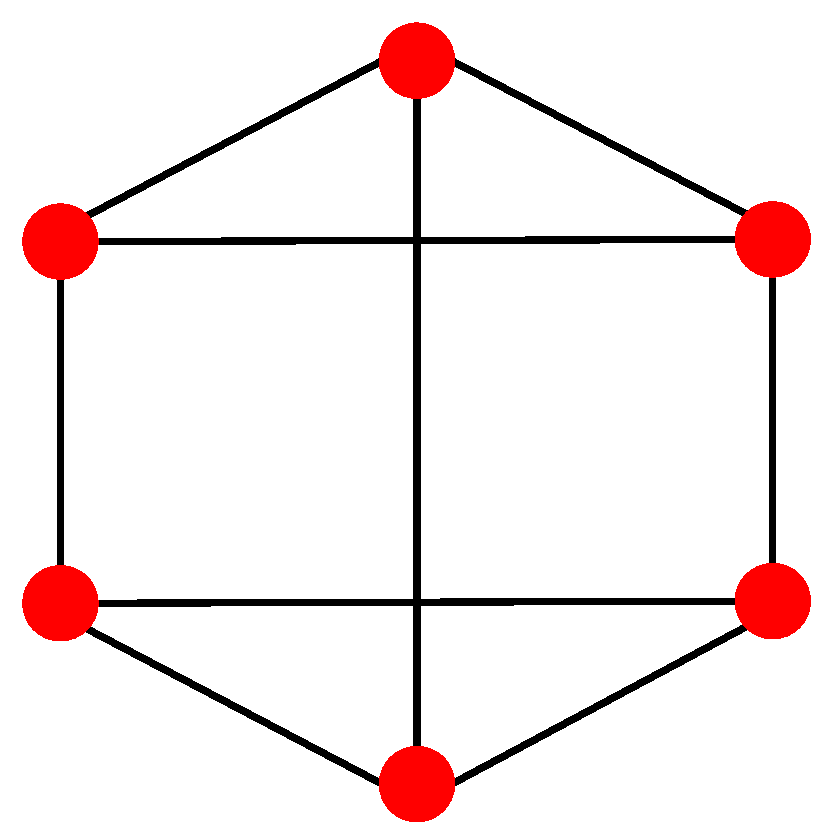
\includegraphics[scale=.2]{../figures/3-regular_graph.pdf}   
        \caption{Example of a 3-regular graph.}         
    \end{minipage}%
    \begin{minipage}{.5\textwidth}
        \centering
        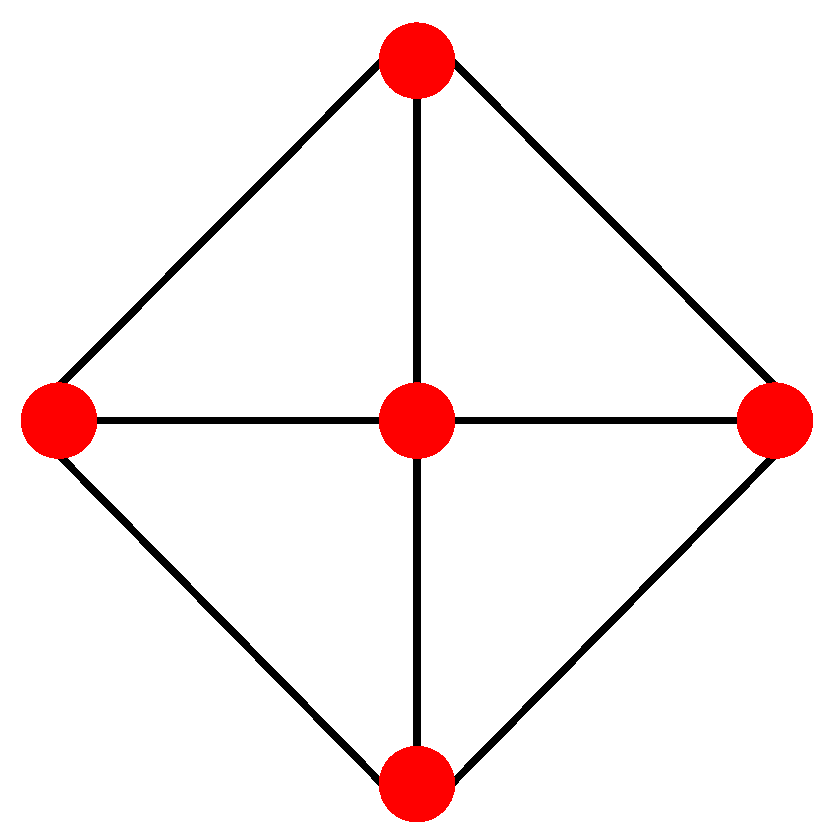
\includegraphics[scale=.2]{../figures/non-regular_graph.pdf}     
        \caption{A non p-regular graph.}       
    \end{minipage}
\end{figure}

We are not going to go as in-depth as we did for the completely connected examples, but we will show
how we can extend OM($m$) to an algorithm that solves the Byzantine Generals Problem with $m $traitors
if the graph of generals, $G$, is $3m$-regular. As a note, a $3m$-regular graph needs to contain at least
$3m+1$ nodes. We will define an algorithm OM($m,p$) that works for all positive integers $m$ and $p$ and with
a regular graph $G$. This algorithm will not work if $G$ is not p-regular.

\noindent\emph{Algorithm OM($m,p$)} \\
\vspace{-10pt}
\begin{enumerate}[label=\arabic{enumi}.]
    \item Choose a regular set $N$ of neighbors of the commander consisting of $p$ lieutenants.
    \item The commander sends their value to every lieutenant in $N$.
    \item {
        For each $i$ in $N$, let $v_i$ be the value Lieutenant $i$ receives from the commander, or else
        RETREAT if they receives no value. Lieutenant $i$ sends $v_i$ to every other lieutenant $k$ as follows:
        \begin{enumerate}[label={\alph*.}]
               \item {
                    If $m = 1$, then by sending the value along the path $\gamma_{i,k}$ whose existence 
                    is guaranteed by the definition of regular set of neighbors.
            }
            \item {
                    If $m>1$, then by acting as the commander in the algorithm OM($m-1, p-1$), with the 
                    graph of generals obtained by removing the original commander from $G$.
            }
        \end{enumerate}
    }
    \item {
        For each $k$, and each $i$ in $N$ with $i \neq k$, let $v_i$ be the value Lieutenant $k$ received from
        Lieutenant $i$ in step (2), or RETREAT if they received no value. Lieutenant $k$ uses the value
        $majority(v_{i1},...,v_{ip})$, where $N = \{i_1,...,i_p\}$.
    }
\end{enumerate}

In the paper the authors go into more detail about this algorithm as well as a way to extend SM($m$)
to handle weakly connected graphs. This is beyond the scope of this paper, as we are focusing on
the Byzantine Generals Problem for completely connected graph. I just wanted to show that the problem
increases in complexity when each general cannot communicate directly with one another. I also wanted
to show an example of how one could approach that problem.

%%%%%%%%%%%%%%%%%%%%%%%%%%%%%%%%%%%%%%%%%%%%%%%%%%%%%%%%%%%%%%%%%%%%%%%%%%%%%%%%%%%%%%%%%%%%%%%%
%%  Conclusion
%%%%%%%%%%%%%%%%%%%%%%%%%%%%%%%%%%%%%%%%%%%%%%%%%%%%%%%%%%%%%%%%%%%%%%%%%%%%%%%%%%%%%%%%%%%%%%%%
\section{Conclusion}

The Byzantine Generals Problem is important in discussing the reliability of computing systems,
especially when it comes to distributed systems. In the real world nothing is perfect, so systems
but be able to handle parts failing, or traitorous generals. A modern application of the problem
is block-chain and Bitcoin. The entire point of Bitcoin is to be decentralized and still reliable.
Whenever a new coin is mined or a transaction is made, other nodes in the Bitcoin network must be
informed and agree that it was legit transaction. If a small number of bad actors were able to
influence whether or not transactions were accepted, then it would lose any credibility it has as a
currency.

Crypto-currency is not the only application of the Byzantine Generals Problem, practically every
network is an example of it in action. Whenever a network cannot afford downtime, the Byzantine
Generals Problem is a fundamental consideration during creation of that network. 

%%%%%%%%%%%%%%%%%%%%%%%%%%%%%%%%%%%%%%%%%%%%%%%%%%%%%%%%%%%%%%%%%%%%%%%%%%%%%%%%%%%%%%%%%%%%%%%%
%%  References
%%%%%%%%%%%%%%%%%%%%%%%%%%%%%%%%%%%%%%%%%%%%%%%%%%%%%%%%%%%%%%%%%%%%%%%%%%%%%%%%%%%%%%%%%%%%%%%%

\bibliographystyle{amsplain}
\begin{thebibliography}{10}

\bibitem{LL} {
    L. Lamport, R. Shostak, and M. Pease, ``The Byzantine Generals Problem'', ACM Transactions on 
    Programming Languages and Systems, Vol. 4, No. 3, 1982, 382-401.
}
\end{thebibliography}

\end{document}
